%%%%%%%%%%%%%%%%%%%%%%%%%%%%%%%%%%%%%%%%%
% Beamer Presentation
% LaTeX Template
% Version 1.0 (10/11/12)
%
% This template has been downloaded from:
% http://www.LaTeXTemplates.com
%
% License:
% CC BY-NC-SA 3.0 (http://creativecommons.org/licenses/by-nc-sa/3.0/)
%
%%%%%%%%%%%%%%%%%%%%%%%%%%%%%%%%%%%%%%%%%

%----------------------------------------------------------------------------------------
%	PACKAGES AND THEMES
%----------------------------------------------------------------------------------------

%\documentclass[UTF8,aspectratio=169,14pt]{ctexbeamer}
\documentclass[UTF8,aspectratio=169]{ctexbeamer}
\usepackage{hyperref}
\hypersetup{
	colorlinks=true,
	linkcolor=red,
	anchorcolor=blue,
	citecolor=green
}

\mode<presentation> {
	
	% The Beamer class comes with a number of default slide themes
	% which change the colors and layouts of slides. Below this is a list
	% of all the themes, uncomment each in turn to see what they look like.
	
	%\usetheme{default}
	%\usetheme{AnnArbor}
	%\usetheme{Antibes}
	%\usetheme{Bergen}
	%\usetheme{Berkeley}
	%\usetheme{Berlin}
	%\usetheme{Boadilla}
	%\usetheme{CambridgeUS}
	%\usetheme{Copenhagen}
	%\usetheme{Darmstadt}
	%\usetheme{Dresden}
	%\usetheme{Frankfurt}
	%\usetheme{Goettingen}
	%\usetheme{Hannover}
	%\usetheme{Ilmenau}
	%\usetheme{JuanLesPins}
	%\usetheme{Luebeck}
	\usetheme{Madrid}
	%\usetheme{Malmoe}
	%\usetheme{Marburg}
	%\usetheme{Montpellier}
	%\usetheme{PaloAlto}
	%\usetheme{Pittsburgh}
	%\usetheme{Rochester}
	%\usetheme{Singapore}
	%\usetheme{Szeged}
	%\usetheme{Warsaw}
	
	% As well as themes, the Beamer class has a number of color themes
	% for any slide theme. Uncomment each of these in turn to see how it
	% changes the colors of your current slide theme.
	
	%\usecolortheme{albatross}
	%\usecolortheme{beaver}
	%\usecolortheme{beetle}
	%\usecolortheme{crane}
	%\usecolortheme{dolphin}
	%\usecolortheme{dove}
	%\usecolortheme{fly}
	%\usecolortheme{lily}
	%\usecolortheme{orchid}
	%\usecolortheme{rose}
	%\usecolortheme{seagull}
	%\usecolortheme{seahorse}
	%\usecolortheme{whale}
	%\usecolortheme{wolverine}
	
	%\setbeamertemplate{footline} % To remove the footer line in all slides uncomment this line
	%\setbeamertemplate{footline}[page number] % To replace the footer line in all slides with a simple slide count uncomment this line
	
	%\setbeamertemplate{navigation symbols}{} % To remove the navigation symbols from the bottom of all slides uncomment this line
}

\usepackage{graphicx} % Allows including images
\graphicspath{{./figs/}}
\usepackage{booktabs} % Allows the use of \toprule, \midrule and \bottomrule in tables
\usepackage{longtable}
\usepackage{listings}
\usepackage{xcolor}
\lstset{numbers=left, %设置行号位置
	numberstyle=\tiny, %设置行号大小
	keywordstyle=\color{blue}, %设置关键字颜色
	commentstyle=\color[cmyk]{1,0,1,0}, %设置注释颜色
	frame=single, %设置边框格式
	escapeinside=``, %逃逸字符(1左面的键),用于显示中文
	%breaklines, %自动折行
	extendedchars=false, %解决代码跨页时,章节标题,页眉等汉字不显示的问题
	xleftmargin=2em,xrightmargin=2em, aboveskip=1em, %设置边距
	tabsize=4, %设置tab空格数
	showspaces=false %不显示空格
}
% Fonts
% \usepackage{libertine}
% \setmonofont{Courier}
\setCJKsansfont[ItalicFont=Noto Serif CJK SC Black, BoldFont=Noto Sans CJK SC Black]{Noto Sans CJK SC}
\setmainfont[Ligatures={Common,TeX}]{Linux  Libertine O}
\setmonofont[SmallCapsFont={Latin Modern Mono Caps}]{Latin Modern Mono Light}
\setsansfont{Linux Biolinum O}

\logo{
\includegraphics[width=0.55cm,height=0.55cm]{../../thcs-logo.png}}

%----------------------------------------------------------------------------------------
%	TITLE PAGE
%----------------------------------------------------------------------------------------

\title[第6讲]{第6讲 :The Programming Languages of OS} % The short title appears at the bottom of every slide, the full title is only on the title page
\subtitle{第四节:The benefits and costs of writing kernel in a high-level language}
\author{陈渝} % Your name
\institute[清华大学] % Your institution as it will appear on the bottom of every slide, may be shorthand to save space
{
	清华大学计算机系 \\ % Your institution for the title page
	\medskip
	\textit{yuchen@tsinghua.edu.cn} % Your email address
}
\date{\today} % Date, can be changed to a custom date


\begin{document}

\begin{frame}
\titlepage % Print the title page as the first slide
\end{frame}

%\begin{frame}
%\frametitle{提纲} % Table of contents slide, comment this block out to remove it
%\tableofcontents % Throughout your presentation, if you choose to use \section{} and \subsection{} commands, these will automatically be printed on this slide as an overview of your presentation
%\end{frame}
%
%%----------------------------------------------------------------------------------
%%	PRESENTATION SLIDES
%%----------------------------------------------------------------------------------------
%
%%------------------------------------------------
%\section{第一节:课程概述} % Sections can be created in order to organize your presentation into discrete blocks, all sections and subsections are automatically printed in the table of contents as an overview of the talk
%%------------------------------------------------

%-------------------------------------------------
\begin{frame}[plain]
	\frametitle{Introduction -- Biscuit}
	
	
	
	\begin{columns}
		
		\begin{column}{.5\textwidth}
			
			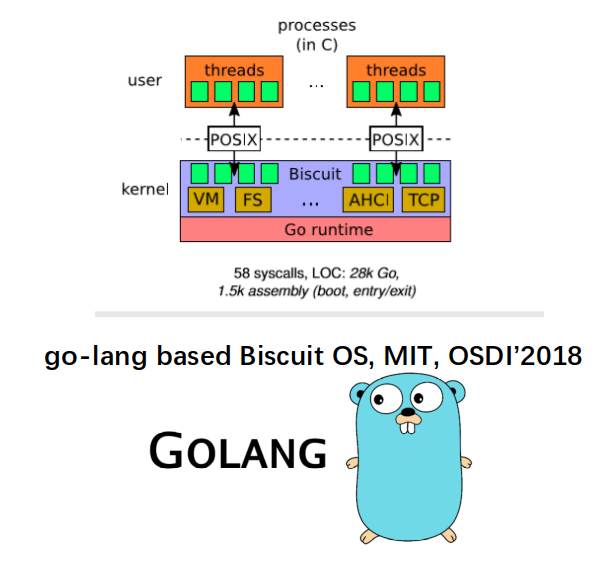
\includegraphics[width=1.\textwidth]{biscuit-intro}
			
		\end{column}
		
		\begin{column}{.5\textwidth}
			
			\Large
		Should we use high-level languages to build
		OS kernels? \\
		
			\normalsize
			Benefits
			\begin{itemize}
				\item Easier to program
				\item Simpler concurrency with GC
				\item Prevents classes of kernel bugs	
			\end{itemize}
			
			Downside
			\begin{itemize}
				\item Bounds, cast, nil-pointer checks
				\item Reflection
				\item Garbage collection	
			\end{itemize}
		\end{column}
		
		
	\end{columns}
	
	
\end{frame}


%-------------------------------------------------
\begin{frame}[plain]
	\frametitle{Introduction -- Biscuit}
	
	
	
	\begin{columns}
		
		\begin{column}{.5\textwidth}
			
			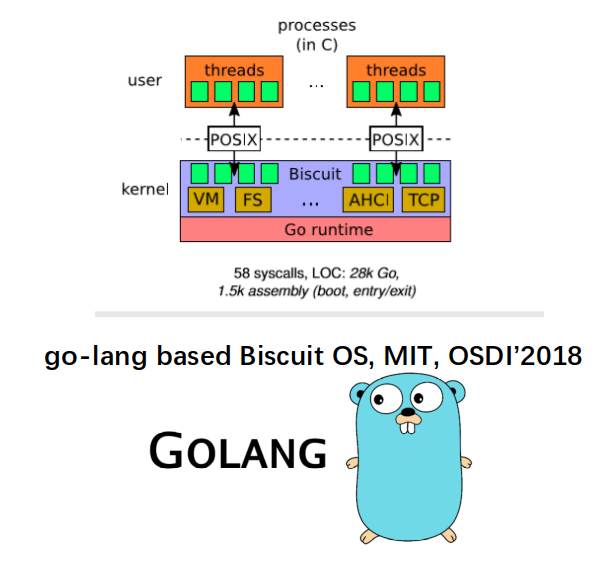
\includegraphics[width=1.\textwidth]{biscuit-intro}
			
		\end{column}
		
		\begin{column}{.5\textwidth}
			
			\Large
	 	  Goal: measure HLL impact  \\
			
			\normalsize
			Pros:
			\begin{itemize}
				\item Reduction of bugs
				\item Simpler code	
			\end{itemize}
			
			Cons:
			\begin{itemize}
				\item HLL safety tax
				\item GC CPU and memory overhead				
				\item GC pause times	
			\end{itemize}
		\end{column}
		
		
	\end{columns}
	
	
\end{frame}

%-------------------------------------------------
\begin{frame}[plain]
	\frametitle{Introduction -- Biscuit}
	
	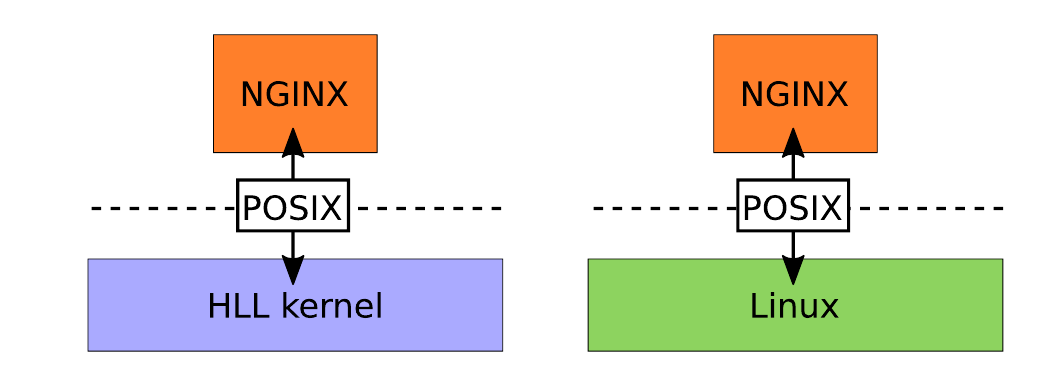
\includegraphics[width=.9\textwidth]{biscuit-method}
	Methodology
	\begin{itemize}
		\item None measure HLL impact in a monolithic POSIX kernel
		\item Build new HLL kernel, compare with Linux
		\item  Isolate HLL impact:
		\item Same apps, POSIX interface, and monolithic organization
		
	\end{itemize}
	
	
\end{frame}


%-------------------------------------------------
\begin{frame}[plain]
	\frametitle{Introduction -- Biscuit}

	\begin{columns}
	
	\begin{column}{.4\textwidth}
		
		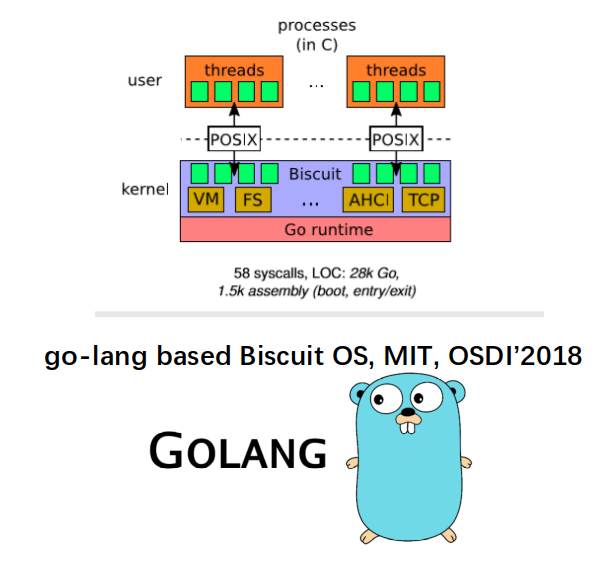
\includegraphics[width=1.\textwidth]{biscuit-intro}
		
		\centering
		58 syscalls, LOC: 28k Go,
		1.5k assembly (boot, entry/exit)
		
	\end{column}
	
	\begin{column}{.6\textwidth}
	Go-lang
	\begin{itemize}
		\item Easy to call asm
		\item Compiled to machine code w/good compiler
		\item  Easy concurrency \& static analysis
		\item GC
		\begin{itemize}
		  \item Concurrent mark and sweep
		  \item Stop-the-world pauses of 10s of μs
		\end{itemize} 
	\end{itemize}
\end{column}
\end{columns}	
\end{frame}


%-------------------------------------------------
\begin{frame}[plain]
	\frametitle{Introduction -- Biscuit}
	
	\begin{columns}
		
		\begin{column}{.4\textwidth}
			
			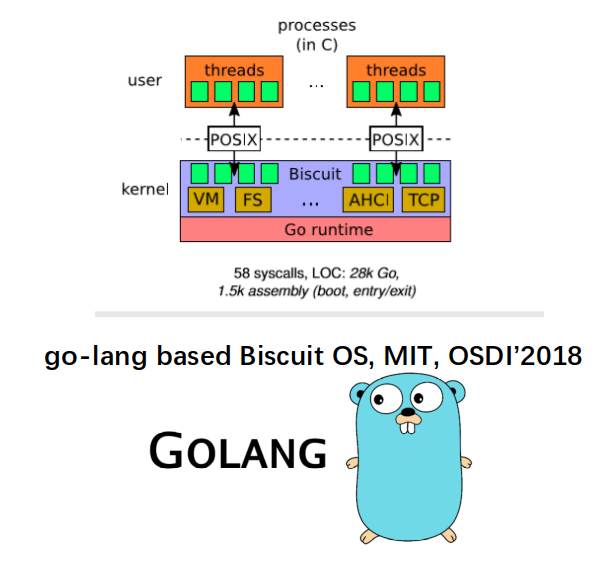
\includegraphics[width=1.\textwidth]{biscuit-intro}
			
			\centering
			58 syscalls, LOC: 28k Go,
			1.5k assembly (boot, entry/exit)
			
		\end{column}
		
		\begin{column}{.6\textwidth}
			Biscuit
			\begin{itemize}
				\item Multicore
				
				\item Threads
				
				\item Journaled FS (7k LOC)
				
				\item Virtual memory (2k LOC)
				\item TCP/IP stack (5k LOC)

				\item Drivers: AHCI and Intel 10G NIC (3k LOC)
				
				
			\end{itemize}
		\end{column}
	\end{columns}	
\end{frame}


%-------------------------------------------------
\begin{frame}[plain]
	\frametitle{Introduction -- Biscuit}
	
	\begin{columns}
		
		\begin{column}{.4\textwidth}
			
			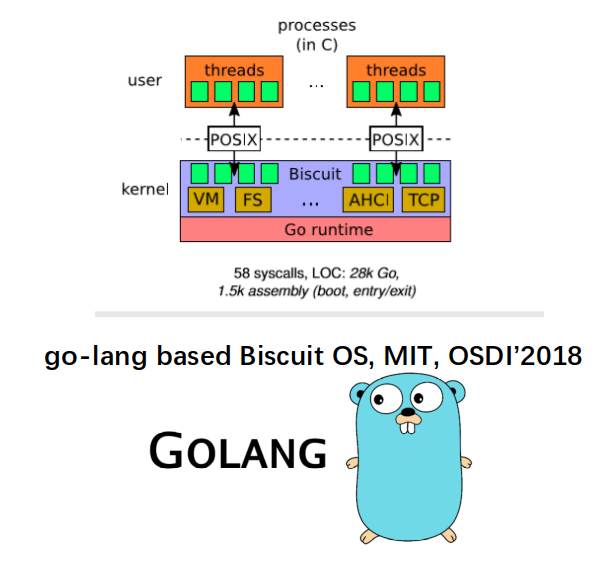
\includegraphics[width=1.\textwidth]{biscuit-intro}
			
			\centering
			58 syscalls, LOC: 28k Go,
			1.5k assembly (boot, entry/exit)
			
		\end{column}
		
		\begin{column}{.6\textwidth}
			Many implementation puzzles in Biscuit
			\begin{itemize}
				\item Interrupts
				\item Threads			
				\item Kernel threads are lightweight	
				\item Runtime on bare-metal
				\item Heap exhaustion (Surprising)
				\item etc.
			\end{itemize}
		\end{column}
	\end{columns}	
\end{frame}


%-------------------------------------------------
\begin{frame}[plain]
	\frametitle{Introduction -- Biscuit}
	
	\begin{columns}
		
		\begin{column}{.4\textwidth}
			
			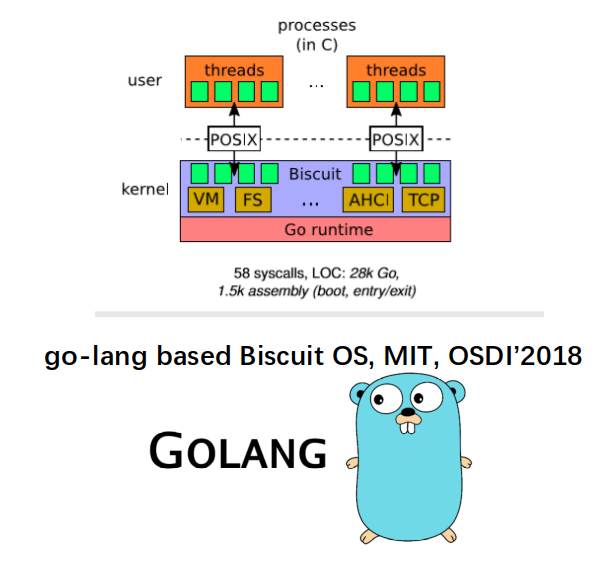
\includegraphics[width=1.\textwidth]{biscuit-intro}
			
			\centering
			58 syscalls, LOC: 28k Go,
			1.5k assembly (boot, entry/exit)
			
		\end{column}
		
		\begin{column}{.6\textwidth}
			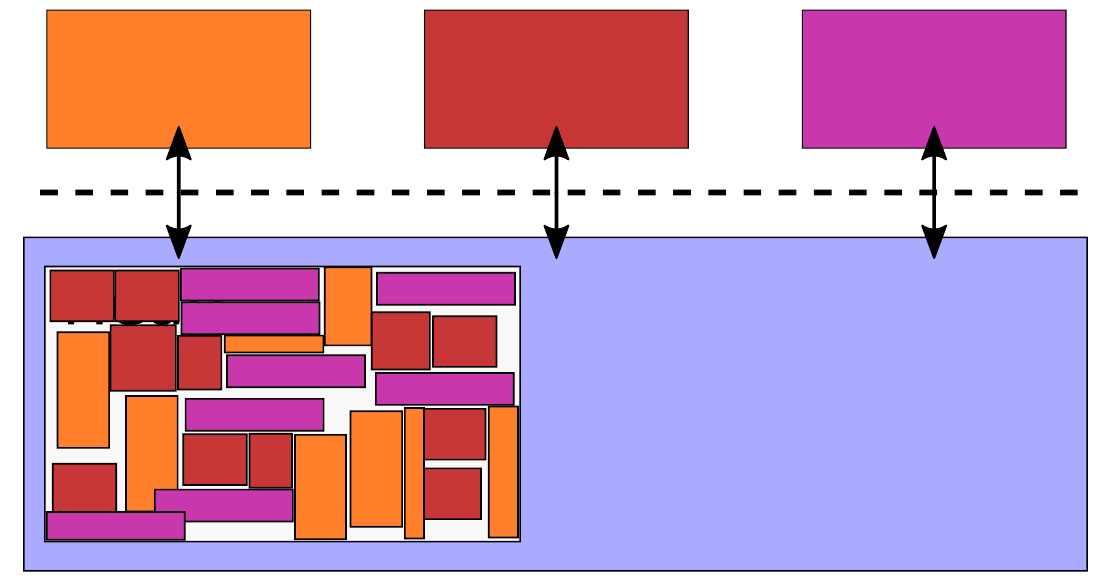
\includegraphics[width=.8\textwidth]{biscuit-heap}
			\begin{itemize}
				\item Can’t allocate heap memory =⇒ nothing works
				\item All kernels face this problem

			\end{itemize}
		\end{column}
	\end{columns}	
\end{frame}

%-------------------------------------------------
\begin{frame}[plain]
	\frametitle{Introduction -- Biscuit}
	
	\begin{columns}
		
		\begin{column}{.4\textwidth}
			
			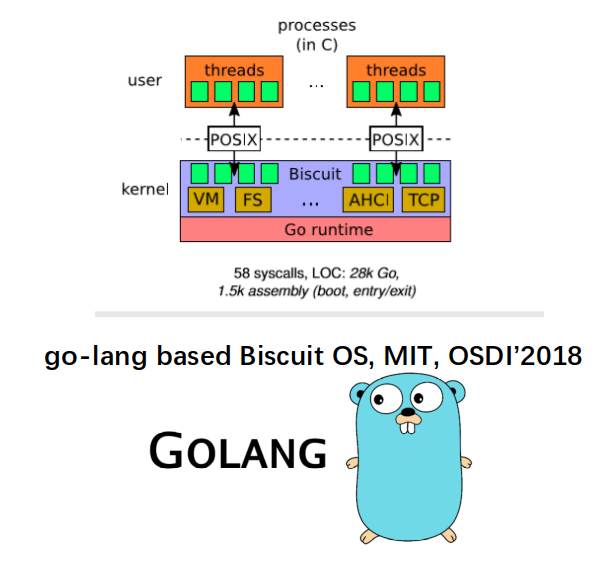
\includegraphics[width=1.\textwidth]{biscuit-intro}
			
			\centering
			58 syscalls, LOC: 28k Go,
			1.5k assembly (boot, entry/exit)
			
		\end{column}
		
		\begin{column}{.6\textwidth}
%			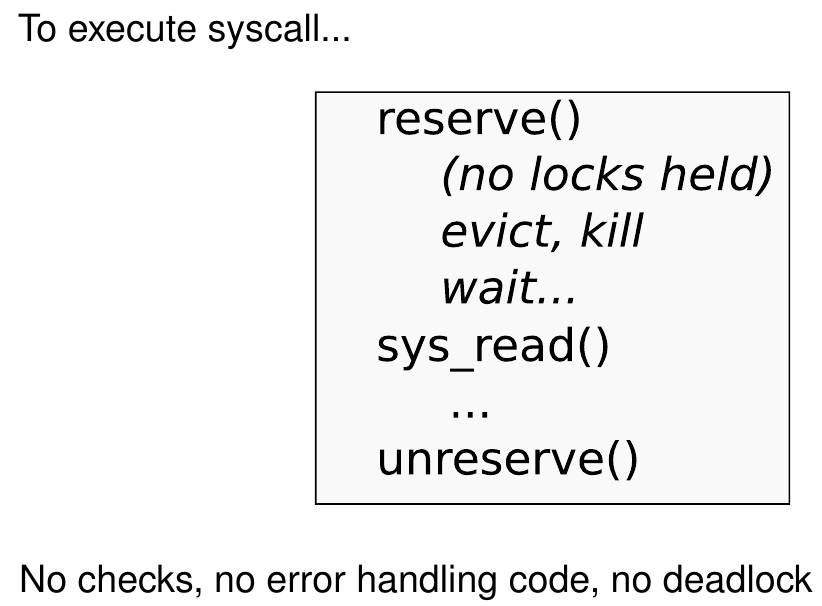
\includegraphics[width=.8\textwidth]{biscuit-heap-solution}
			Strawman 1: Wait for memory in allocator?

			\begin{itemize}
				\item May deadlock!
				
		    \end{itemize}	
	    
	        Strawman 2: Check/handle allocation failure, like C kernels?
	        
	        \begin{itemize}
				\item Difficult to get right
				\item Can’t! Go doesn’t expose failed allocations
				\item and implicitly allocates
		
			\end{itemize}
		Both cause problems for Linux; see “too small to fail” rule
		
		\end{column}
	\end{columns}	
\end{frame}

%-------------------------------------------------
\begin{frame}[plain]
	\frametitle{Introduction -- Biscuit}
	
	\begin{columns}
		
		\begin{column}{.4\textwidth}
			
			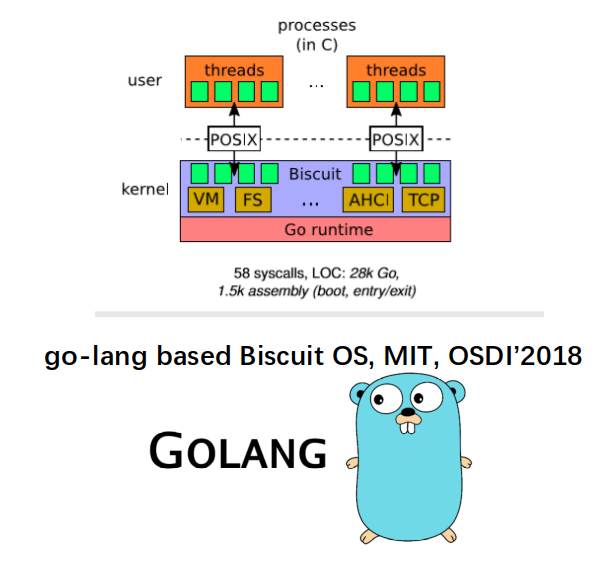
\includegraphics[width=1.\textwidth]{biscuit-intro}
			
			\centering
			58 syscalls, LOC: 28k Go,
			1.5k assembly (boot, entry/exit)
			
		\end{column}
		
		\begin{column}{.6\textwidth}
			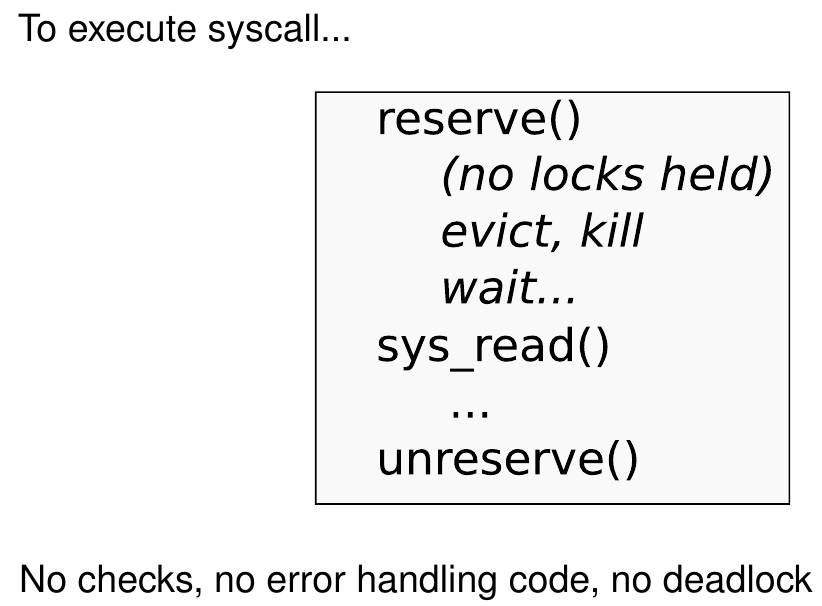
\includegraphics[width=.8\textwidth]{biscuit-heap-solution}
			Reservations
			
			\begin{itemize}
				\item HLL easy to analyze
				
				\item Tool computes reservation via escape analysis
				
				\item ≈ three days of expert effort to apply tool
				
			\end{itemize}
		\end{column}
	\end{columns}	
\end{frame}



%-------------------------------------------------
\begin{frame}[plain]
	\frametitle{Introduction -- Biscuit}
	
	\begin{columns}
		
		\begin{column}{.4\textwidth}
			
			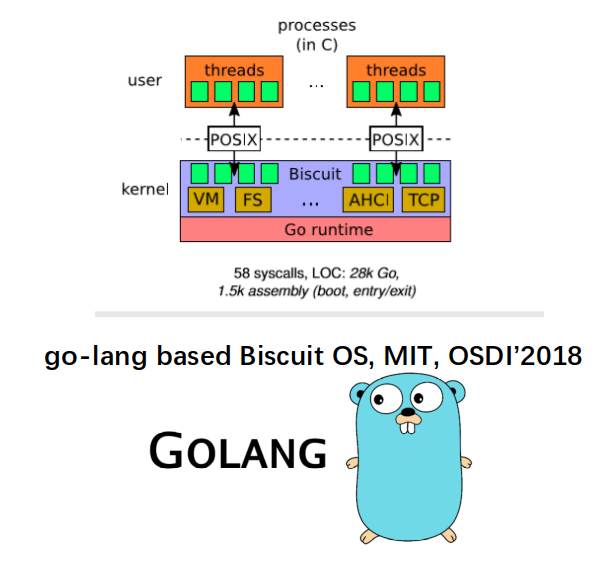
\includegraphics[width=1.\textwidth]{biscuit-intro}
			
			\centering
			58 syscalls, LOC: 28k Go,
			1.5k assembly (boot, entry/exit)
			
		\end{column}
		
		\begin{column}{.6\textwidth}
			BISCUIT adopted many Linux optimizations:
			
			\begin{itemize}
				\item large pages for kernel text
				\item per-CPU NIC transmit queues
				\item RCU-like directory cache
				\item concurrent FS transactions
				\item pad structs to remove false sharing
				
			\end{itemize}
		Good OS performance more about optimizations, less about HLL
		
		\end{column}
	\end{columns}	
\end{frame}



%-------------------------------------------------
\begin{frame}[plain]
	\frametitle{Introduction -- Biscuit}
	
	\begin{columns}
		
		\begin{column}{.4\textwidth}
			
			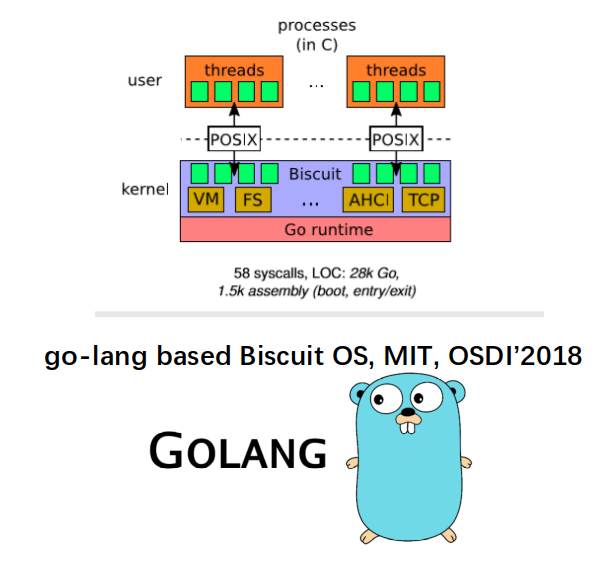
\includegraphics[width=1.\textwidth]{biscuit-intro}
			
			\centering
			58 syscalls, LOC: 28k Go,
			1.5k assembly (boot, entry/exit)
			
		\end{column}
		
		\begin{column}{.6\textwidth}
		Eval: Should we use high-level languages to build OS kernels?
			\begin{itemize}
				\item Did B ISCUIT benefit from HLL features?
				
				\item  Is B ISCUIT performance in the same league as Linux?
				
				\item What is the breakdown of HLL tax?
				
				\item  What is the performance cost of Go compared to C?
				
				
			\end{itemize}
			
			
		\end{column}
	\end{columns}	
\end{frame}


%-------------------------------------------------
\begin{frame}[plain]
	\frametitle{Introduction -- Biscuit}
	
	\begin{columns}
		
		\begin{column}{.4\textwidth}
			
			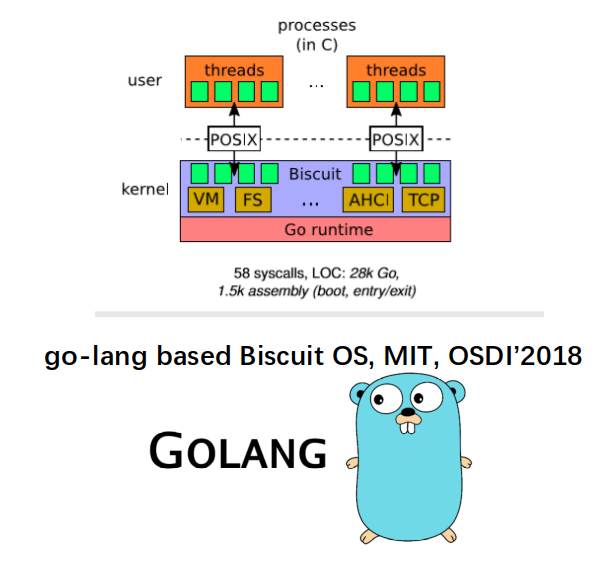
\includegraphics[width=1.\textwidth]{biscuit-intro}
			
			\centering
			58 syscalls, LOC: 28k Go,
			1.5k assembly (boot, entry/exit)
			
		\end{column}
		
		\begin{column}{.6\textwidth}
			Eval:  Qualitative benefits of HLL features
			
			\begin{itemize}
				\item GC’ed allocation
				
				
				\item  defer
				
				
				\item multi-valued return
				
				
				\item  closures
				
				\item maps
				
			\end{itemize}
		Inspected fixes for all publicly-available execute code CVEs in
		Linux kernel for 2017
		
			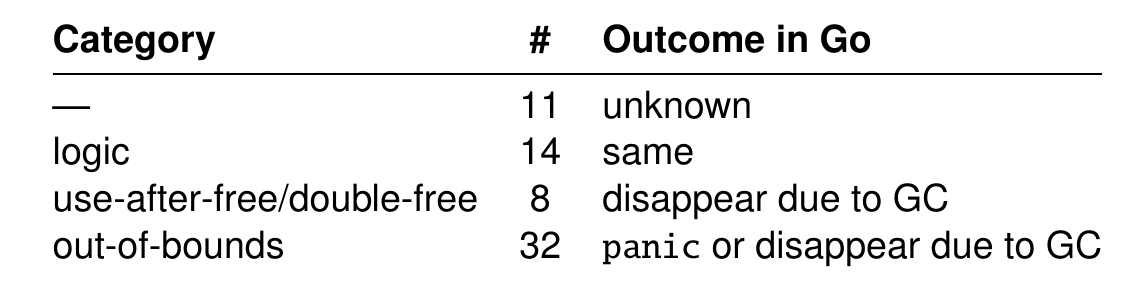
\includegraphics[width=.9\textwidth]{biscuit-nobug}
			panic likely better than malicious code execution
			
		\end{column}
	\end{columns}	
\end{frame}



%-------------------------------------------------
\begin{frame}[plain]
	\frametitle{Introduction -- Biscuit}
	\centering
 Biscuit and Linux in the same league	
 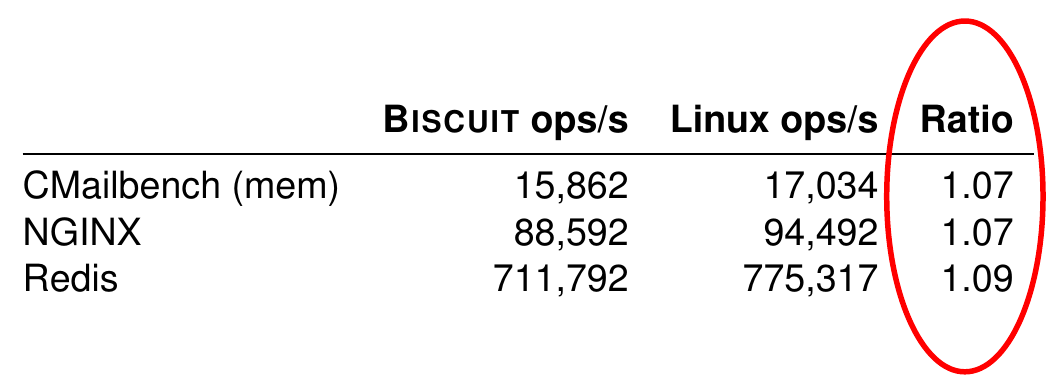
\includegraphics[width=.7\textwidth]{biscuit-benchs}
 
  the breakdown of HLL tax in Biscuit
 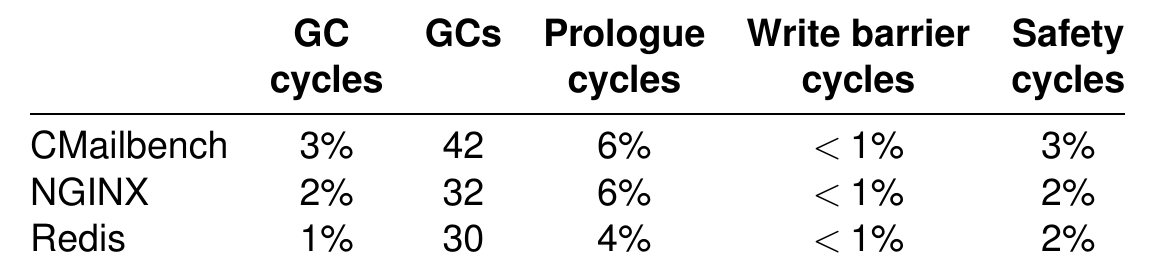
\includegraphics[width=.7\textwidth]{biscuit-hll-tax}
%Benchmarks allocate kernel heap rapidly
%but have little persistent kernel heap data
%Cycles used by GC increase with size of live kernel heap
%Dedicate 2 or 3× memory ⇒ low GC cycles

\end{frame}

%-------------------------------------------------
\begin{frame}[plain]
	\frametitle{Introduction -- Biscuit}
	\centering
	C is 15\% faster \\
	Prologue/safety-checks ⇒ 16\% more instructions
		
	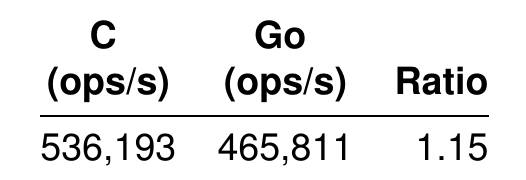
\includegraphics[width=.5\textwidth]{biscuit-speed}
	
	\begin{itemize}
	
	\item The HLL worked well for kernel development
	
	\item Performance is paramount ⇒ use C (up to 15\%)
	
	\item Minimize memory use ⇒ use C (↓ mem. budget, ↑ GC cost)
	
	\item Safety is paramount ⇒ use HLL (40 CVEs stopped)
	
	\item Performance merely important ⇒ use HLL (pay 15\%, memory)
	
\end{itemize}
	
\end{frame}
%-------------------------------------------------
\begin{frame}[plain]
	\frametitle{References}

	\begin{itemize}

		\item Multiprogramming a 64 kB Computer Safely and Efficiently,SOSP 2017
		\item  The benefits and costs of writing a POSIX
		kernel in a high-level language
		,OSDI 2018
		
	\end{itemize}
	
	
\end{frame}
%-------------------------------------------------
%-------------------------------------------------
\end{document}